\documentclass{standalone}
\usepackage{tikz}
\usetikzlibrary{patterns, positioning}


\begin{document}
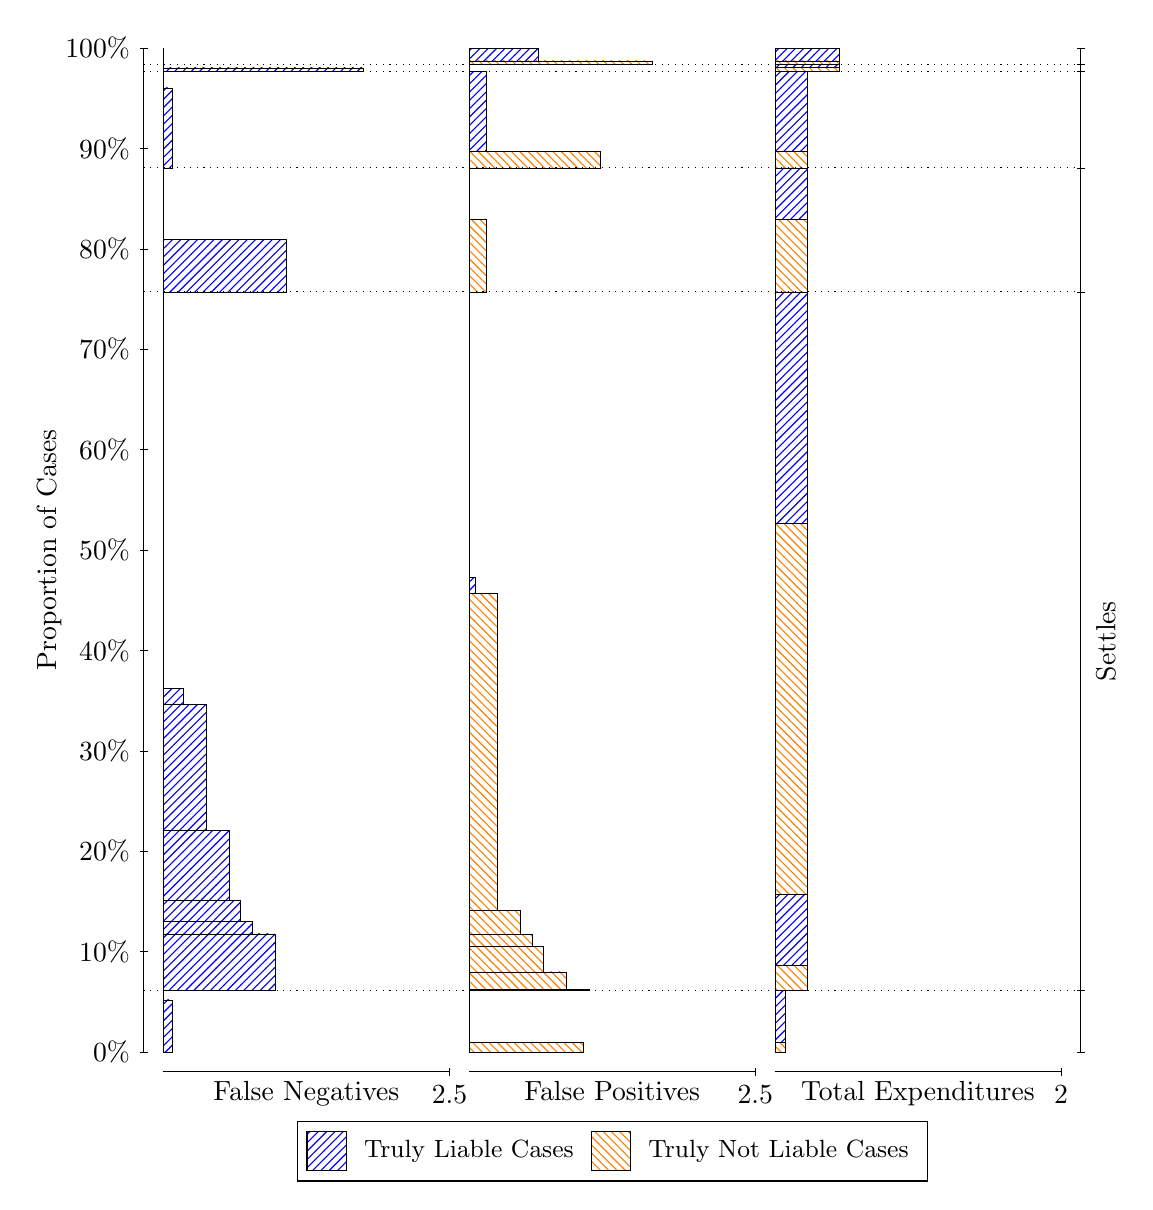
\begin{tikzpicture}
\draw[black, very thin] (1.5,1.75) -- (1.5,14.5);
\node[rotate=90, text=black, anchor=center] at (0.3, 8.125) {Proportion of Cases};
\draw[black, very thin] (1.45,1.75) -- (1.55,1.75);
\node[text=black, anchor=east] at (1.45, 1.75) {0\%};
\draw[black, very thin] (1.45,3.025) -- (1.55,3.025);
\node[text=black, anchor=east] at (1.45, 3.025) {10\%};
\draw[black, very thin] (1.45,4.3) -- (1.55,4.3);
\node[text=black, anchor=east] at (1.45, 4.3) {20\%};
\draw[black, very thin] (1.45,5.575) -- (1.55,5.575);
\node[text=black, anchor=east] at (1.45, 5.575) {30\%};
\draw[black, very thin] (1.45,6.85) -- (1.55,6.85);
\node[text=black, anchor=east] at (1.45, 6.85) {40\%};
\draw[black, very thin] (1.45,8.125) -- (1.55,8.125);
\node[text=black, anchor=east] at (1.45, 8.125) {50\%};
\draw[black, very thin] (1.45,9.4) -- (1.55,9.4);
\node[text=black, anchor=east] at (1.45, 9.4) {60\%};
\draw[black, very thin] (1.45,10.675) -- (1.55,10.675);
\node[text=black, anchor=east] at (1.45, 10.675) {70\%};
\draw[black, very thin] (1.45,11.95) -- (1.55,11.95);
\node[text=black, anchor=east] at (1.45, 11.95) {80\%};
\draw[black, very thin] (1.45,13.225) -- (1.55,13.225);
\node[text=black, anchor=east] at (1.45, 13.225) {90\%};
\draw[black, very thin] (1.45,14.5) -- (1.55,14.5);
\node[text=black, anchor=east] at (1.45, 14.5) {100\%};

\draw[black, very thin] (13.4,1.75) -- (13.4,14.5);
\draw[black, very thin] (13.35,1.75) -- (13.45,1.75);
\node[anchor=west] at (13.35, 1.75) {};
\draw[black, very thin] (13.35,2.5315) -- (13.45,2.5315);
\node[anchor=west] at (13.35, 2.5315) {};
\draw[black, very thin] (13.35,11.404) -- (13.45,11.404);
\node[anchor=west] at (13.35, 11.404) {};
\draw[black, very thin] (13.35,12.979) -- (13.45,12.979);
\node[anchor=west] at (13.35, 12.979) {};
\draw[black, very thin] (13.35,14.204) -- (13.45,14.204);
\node[anchor=west] at (13.35, 14.204) {};
\draw[black, very thin] (13.35,14.295) -- (13.45,14.295);
\node[anchor=west] at (13.35, 14.295) {};
\draw[black, very thin] (13.35,14.5) -- (13.45,14.5);
\node[anchor=west] at (13.35, 14.5) {};

\draw[black, very thin, pattern color=blue, pattern=north east lines] (1.75,1.75) rectangle (1.859,2.4107);
\draw[black, very thin, pattern color=orange, pattern=north west lines] (1.75,2.4107) rectangle (1.75,2.5315);
\draw[black, very thin, pattern color=blue, pattern=north east lines] (1.75,2.5315) rectangle (3.167,3.2495);
\draw[black, very thin, pattern color=blue, pattern=north east lines] (1.75,3.2495) rectangle (2.8763,3.406);
\draw[black, very thin, pattern color=blue, pattern=north east lines] (1.75,3.406) rectangle (2.731,3.6705);
\draw[black, very thin, pattern color=blue, pattern=north east lines] (1.75,3.6705) rectangle (2.5857,4.5646);
\draw[black, very thin, pattern color=blue, pattern=north east lines] (1.75,4.5646) rectangle (2.295,6.162);
\draw[black, very thin, pattern color=blue, pattern=north east lines] (1.75,6.162) rectangle (2.0043,6.3654);
\draw[black, very thin, pattern color=orange, pattern=north west lines] (1.75,6.3654) rectangle (1.75,11.404);
\draw[black, very thin, pattern color=blue, pattern=north east lines] (1.75,11.404) rectangle (3.3123,12.065);
\draw[black, very thin, pattern color=orange, pattern=north west lines] (1.75,12.065) rectangle (1.75,12.979);
\draw[black, very thin, pattern color=blue, pattern=north east lines] (1.75,12.979) rectangle (1.859,13.994);
\draw[black, very thin, pattern color=orange, pattern=north west lines] (1.75,13.994) rectangle (1.75,14.204);
\draw[black, very thin, pattern color=blue, pattern=north east lines] (1.75,14.204) rectangle (4.2933,14.247);
\draw[black, very thin, pattern color=orange, pattern=north west lines] (1.75,14.247) rectangle (1.75,14.295);
\draw[black, very thin, pattern color=orange, pattern=north west lines] (1.75,14.295) rectangle (1.75,14.338);
\draw[black, very thin, pattern color=blue, pattern=north east lines] (1.75,14.338) rectangle (1.75,14.5);
\draw[black, very thin, pattern color=orange, pattern=north west lines] (5.6333,1.75) rectangle (7.0867,1.8708);
\draw[black, very thin, pattern color=blue, pattern=north east lines] (5.6333,1.8708) rectangle (5.6333,2.5315);
\draw[black, very thin, pattern color=orange, pattern=north west lines] (5.6333,2.5315) rectangle (7.1593,2.5461);
\draw[black, very thin, pattern color=orange, pattern=north west lines] (5.6333,2.5461) rectangle (6.8687,2.766);
\draw[black, very thin, pattern color=orange, pattern=north west lines] (5.6333,2.766) rectangle (6.578,3.0899);
\draw[black, very thin, pattern color=orange, pattern=north west lines] (5.6333,3.0899) rectangle (6.4327,3.2448);
\draw[black, very thin, pattern color=orange, pattern=north west lines] (5.6333,3.2448) rectangle (6.2873,3.5447);
\draw[black, very thin, pattern color=orange, pattern=north west lines] (5.6333,3.5447) rectangle (5.9967,7.57);
\draw[black, very thin, pattern color=blue, pattern=north east lines] (5.6333,7.57) rectangle (5.706,7.7734);
\draw[black, very thin, pattern color=blue, pattern=north east lines] (5.6333,7.7734) rectangle (5.6333,11.404);
\draw[black, very thin, pattern color=orange, pattern=north west lines] (5.6333,11.404) rectangle (5.8513,12.319);
\draw[black, very thin, pattern color=blue, pattern=north east lines] (5.6333,12.319) rectangle (5.6333,12.979);
\draw[black, very thin, pattern color=orange, pattern=north west lines] (5.6333,12.979) rectangle (7.3047,13.189);
\draw[black, very thin, pattern color=blue, pattern=north east lines] (5.6333,13.189) rectangle (5.8513,14.204);
\draw[black, very thin, pattern color=orange, pattern=north west lines] (5.6333,14.204) rectangle (5.6333,14.252);
\draw[black, very thin, pattern color=blue, pattern=north east lines] (5.6333,14.252) rectangle (5.6333,14.295);
\draw[black, very thin, pattern color=orange, pattern=north west lines] (5.6333,14.295) rectangle (7.9587,14.338);
\draw[black, very thin, pattern color=blue, pattern=north east lines] (5.6333,14.338) rectangle (6.5053,14.5);
\draw[black, very thin, pattern color=orange, pattern=north west lines] (9.5167,1.75) rectangle (9.6529,1.8708);
\draw[black, very thin, pattern color=blue, pattern=north east lines] (9.5167,1.8708) rectangle (9.6529,2.5315);
\draw[black, very thin, pattern color=orange, pattern=north west lines] (9.5167,2.5315) rectangle (9.9254,2.8554);
\draw[black, very thin, pattern color=blue, pattern=north east lines] (9.5167,2.8554) rectangle (9.9254,3.7496);
\draw[black, very thin, pattern color=orange, pattern=north west lines] (9.5167,3.7496) rectangle (9.9254,8.4641);
\draw[black, very thin, pattern color=blue, pattern=north east lines] (9.5167,8.4641) rectangle (9.9254,11.404);
\draw[black, very thin, pattern color=orange, pattern=north west lines] (9.5167,11.404) rectangle (9.9254,12.319);
\draw[black, very thin, pattern color=blue, pattern=north east lines] (9.5167,12.319) rectangle (9.9254,12.979);
\draw[black, very thin, pattern color=orange, pattern=north west lines] (9.5167,12.979) rectangle (9.9254,13.189);
\draw[black, very thin, pattern color=blue, pattern=north east lines] (9.5167,13.189) rectangle (9.9254,14.204);
\draw[black, very thin, pattern color=orange, pattern=north west lines] (9.5167,14.204) rectangle (10.334,14.252);
\draw[black, very thin, pattern color=blue, pattern=north east lines] (9.5167,14.252) rectangle (10.334,14.295);
\draw[black, very thin, pattern color=orange, pattern=north west lines] (9.5167,14.295) rectangle (10.334,14.338);
\draw[black, very thin, pattern color=blue, pattern=north east lines] (9.5167,14.338) rectangle (10.334,14.5);
\draw[black, dotted] (1.5,2.5315) -- (13.4,2.5315);
\draw[black, dotted] (1.5,11.404) -- (13.4,11.404);
\draw[black, dotted] (1.5,12.979) -- (13.4,12.979);
\draw[black, dotted] (1.5,14.204) -- (13.4,14.204);
\draw[black, dotted] (1.5,14.295) -- (13.4,14.295);
\draw[black, very thin] (1.75,1.5) -- (5.3833,1.5);
\node[text=black, anchor=north] at (3.5667, 1.5) {False Negatives};
\draw[black, very thin] (5.3833,1.45) -- (5.3833,1.55);
\node[text=black, anchor=north] at (5.3833, 1.45) {2.5};

\draw[black, very thin] (5.6333,1.5) -- (9.2667,1.5);
\node[text=black, anchor=north] at (7.45, 1.5) {False Positives};
\draw[black, very thin] (9.2667,1.45) -- (9.2667,1.55);
\node[text=black, anchor=north] at (9.2667, 1.45) {2.5};

\draw[black, very thin] (9.5167,1.5) -- (13.15,1.5);
\node[text=black, anchor=north] at (11.333, 1.5) {Total Expenditures};
\draw[black, very thin] (13.15,1.45) -- (13.15,1.55);
\node[text=black, anchor=north] at (13.15, 1.45) {2};


\node[text=black, centered, rotate=90] at (13.72, 6.9677) {Settles};





\draw (7.449999999999999,1.5) node[draw=none] (baseCoordinate) {};
\begin{scope}[align=center]
        \matrix[scale=0.5, draw=black, below=0.5cm of baseCoordinate, nodes={draw}, column sep=0.1cm]{
            \node[rectangle, draw, minimum width=0.5cm, minimum height=0.5cm, pattern color=blue, pattern=north east lines] {}; &
            \node[draw=none, font=\small, text=black] (B) {Truly Liable Cases}; &
            \node[rectangle, draw, minimum width=0.5cm, minimum height=0.5cm, pattern color=orange, pattern=north west lines] {}; &
            \node[draw=none, font=\small, text=black] (B) {Truly Not Liable Cases}; \\
            };
\end{scope}

\end{tikzpicture}
\end{document}